% Options for packages loaded elsewhere
\PassOptionsToPackage{unicode}{hyperref}
\PassOptionsToPackage{hyphens}{url}
\PassOptionsToPackage{dvipsnames,svgnames,x11names}{xcolor}
%
\documentclass[
  11pt,
  letterpaper,
  DIV=11,
  numbers=noendperiod]{scrartcl}

\usepackage{amsmath,amssymb}
\usepackage{iftex}
\ifPDFTeX
  \usepackage[T1]{fontenc}
  \usepackage[utf8]{inputenc}
  \usepackage{textcomp} % provide euro and other symbols
\else % if luatex or xetex
  \usepackage{unicode-math}
  \defaultfontfeatures{Scale=MatchLowercase}
  \defaultfontfeatures[\rmfamily]{Ligatures=TeX,Scale=1}
\fi
\usepackage{lmodern}
\ifPDFTeX\else  
    % xetex/luatex font selection
\fi
% Use upquote if available, for straight quotes in verbatim environments
\IfFileExists{upquote.sty}{\usepackage{upquote}}{}
\IfFileExists{microtype.sty}{% use microtype if available
  \usepackage[]{microtype}
  \UseMicrotypeSet[protrusion]{basicmath} % disable protrusion for tt fonts
}{}
\makeatletter
\@ifundefined{KOMAClassName}{% if non-KOMA class
  \IfFileExists{parskip.sty}{%
    \usepackage{parskip}
  }{% else
    \setlength{\parindent}{0pt}
    \setlength{\parskip}{6pt plus 2pt minus 1pt}}
}{% if KOMA class
  \KOMAoptions{parskip=half}}
\makeatother
\usepackage{xcolor}
\setlength{\emergencystretch}{3em} % prevent overfull lines
\setcounter{secnumdepth}{-\maxdimen} % remove section numbering
% Make \paragraph and \subparagraph free-standing
\makeatletter
\ifx\paragraph\undefined\else
  \let\oldparagraph\paragraph
  \renewcommand{\paragraph}{
    \@ifstar
      \xxxParagraphStar
      \xxxParagraphNoStar
  }
  \newcommand{\xxxParagraphStar}[1]{\oldparagraph*{#1}\mbox{}}
  \newcommand{\xxxParagraphNoStar}[1]{\oldparagraph{#1}\mbox{}}
\fi
\ifx\subparagraph\undefined\else
  \let\oldsubparagraph\subparagraph
  \renewcommand{\subparagraph}{
    \@ifstar
      \xxxSubParagraphStar
      \xxxSubParagraphNoStar
  }
  \newcommand{\xxxSubParagraphStar}[1]{\oldsubparagraph*{#1}\mbox{}}
  \newcommand{\xxxSubParagraphNoStar}[1]{\oldsubparagraph{#1}\mbox{}}
\fi
\makeatother


\providecommand{\tightlist}{%
  \setlength{\itemsep}{0pt}\setlength{\parskip}{0pt}}\usepackage{longtable,booktabs,array}
\usepackage{calc} % for calculating minipage widths
% Correct order of tables after \paragraph or \subparagraph
\usepackage{etoolbox}
\makeatletter
\patchcmd\longtable{\par}{\if@noskipsec\mbox{}\fi\par}{}{}
\makeatother
% Allow footnotes in longtable head/foot
\IfFileExists{footnotehyper.sty}{\usepackage{footnotehyper}}{\usepackage{footnote}}
\makesavenoteenv{longtable}
\usepackage{graphicx}
\makeatletter
\def\maxwidth{\ifdim\Gin@nat@width>\linewidth\linewidth\else\Gin@nat@width\fi}
\def\maxheight{\ifdim\Gin@nat@height>\textheight\textheight\else\Gin@nat@height\fi}
\makeatother
% Scale images if necessary, so that they will not overflow the page
% margins by default, and it is still possible to overwrite the defaults
% using explicit options in \includegraphics[width, height, ...]{}
\setkeys{Gin}{width=\maxwidth,height=\maxheight,keepaspectratio}
% Set default figure placement to htbp
\makeatletter
\def\fps@figure{htbp}
\makeatother

\usepackage{booktabs}
\usepackage{longtable}
\usepackage{array}
\usepackage{multirow}
\usepackage{wrapfig}
\usepackage{float}
\usepackage{colortbl}
\usepackage{pdflscape}
\usepackage{tabu}
\usepackage{threeparttable}
\usepackage{threeparttablex}
\usepackage[normalem]{ulem}
\usepackage{makecell}
\usepackage{xcolor}
\renewcommand{\baselinestretch}{1.1}
\usepackage{graphicx}
\usepackage{xcolor}
\usepackage{amsmath,amssymb}
\usepackage{booktabs}
\usepackage{longtable}
\usepackage{array}
\usepackage{multirow}
\usepackage{makecell}
\usepackage{pdflscape}
\usepackage{float}
\usepackage{fancyhdr}
\KOMAoption{captions}{tableheading}
\makeatletter
\@ifpackageloaded{caption}{}{\usepackage{caption}}
\AtBeginDocument{%
\ifdefined\contentsname
  \renewcommand*\contentsname{Table of contents}
\else
  \newcommand\contentsname{Table of contents}
\fi
\ifdefined\listfigurename
  \renewcommand*\listfigurename{List of Figures}
\else
  \newcommand\listfigurename{List of Figures}
\fi
\ifdefined\listtablename
  \renewcommand*\listtablename{List of Tables}
\else
  \newcommand\listtablename{List of Tables}
\fi
\ifdefined\figurename
  \renewcommand*\figurename{Figure}
\else
  \newcommand\figurename{Figure}
\fi
\ifdefined\tablename
  \renewcommand*\tablename{Table}
\else
  \newcommand\tablename{Table}
\fi
}
\@ifpackageloaded{float}{}{\usepackage{float}}
\floatstyle{ruled}
\@ifundefined{c@chapter}{\newfloat{codelisting}{h}{lop}}{\newfloat{codelisting}{h}{lop}[chapter]}
\floatname{codelisting}{Listing}
\newcommand*\listoflistings{\listof{codelisting}{List of Listings}}
\makeatother
\makeatletter
\makeatother
\makeatletter
\@ifpackageloaded{caption}{}{\usepackage{caption}}
\@ifpackageloaded{subcaption}{}{\usepackage{subcaption}}
\makeatother

\ifLuaTeX
  \usepackage{selnolig}  % disable illegal ligatures
\fi
\usepackage{bookmark}

\IfFileExists{xurl.sty}{\usepackage{xurl}}{} % add URL line breaks if available
\urlstyle{same} % disable monospaced font for URLs
\hypersetup{
  pdftitle={LDA Homework 3 (2025-2026)},
  pdfauthor={Anita Kerubo Ogero (2469491); Okolie Tess Eucharia (2468507); Moses Mburu (2469245); Dorothy Chepkoech (2469284)},
  colorlinks=true,
  linkcolor={blue},
  filecolor={Maroon},
  citecolor={Blue},
  urlcolor={Blue},
  pdfcreator={LaTeX via pandoc}}


\title{LDA Homework 3 (2025-2026)}
\author{Anita Kerubo Ogero (2469491) \and Okolie Tess Eucharia
(2468507) \and Moses Mburu (2469245) \and Dorothy Chepkoech (2469284)}
\date{}

\begin{document}
\maketitle


\subsection{Methodology}\label{methodology}

\subsubsection{Notation and data
structure}\label{notation-and-data-structure}

Let \(i=1,\dots,N\) index patients and \(j=0,\dots,J\) index scheduled
annual visits (\(j=0\) baseline). The continuous outcome of interest is
the BPRS score \(Y_{ij}\). Define the missingness indicator

\[
R_{ij} =
\begin{cases}
1, & \text{if } Y_{ij}\ \text{is observed},\
0, & \text{if } Y_{ij}\ \text{is missing.}
\end{cases}
\]

Let \(R_i=(R_{i0},\dots,R_{iJ})\) denote the subject-specific
observation pattern, and split the full outcome vector as
\(Y_i=(Y_i^{obs},Y_i^{mis})\).

\subsubsection{Missingness pattern and dropout
taxonomy}\label{missingness-pattern-and-dropout-taxonomy}

The first goal is to describe whether missingness behaves like monotone
dropout (typical in longitudinal follow-up) or intermittent missingness
(temporary gaps). For each patient:

\begin{enumerate}
\def\labelenumi{\arabic{enumi}.}
\item
  \textbf{Completeness.} A patient is complete if \(R_{ij}=1\) for all
  \(j\).
\item
  \textbf{Monotone missingness (dropout-type).} Define the last observed
  visit \[
  t_i=\max{j: R_{ij}=1}.
  \]

  The pattern is monotone if

  \[
  R_{ij}=1 \text{ for } j\le t_i,\qquad R_{ij}=0 \text{ for } j>t_i.
  \]
\item
  \textbf{Non-monotone (intermittent) missingness.} The pattern is
  non-monotone if there exist \(j<k\) such that \[
  R_{ij}=0 \ \text{and}\ R_{ik}=1.
  \]
\end{enumerate}

These classifications are summarised using (i) the distribution of
\(t_i\) (retention over time), (ii) the proportion missing at each visit
\(j\), and (iii) the frequency of intermittent gaps within \(R_i\). In
this Alzheimer cohort, missingness rises markedly with follow-up, so
later-visit summaries are based on a progressively smaller subset of
participants.

\subsubsection{Proportion missing by
time}\label{proportion-missing-by-time}

\begin{verbatim}
    time n_total n_obs n_miss prop_miss
   <int>   <int> <int>  <int>     <num>
1:     0    1253  1253      0 0.0000000
2:     1    1253  1106    147 0.1173184
3:     2    1253  1014    239 0.1907422
4:     3    1253   907    346 0.2761373
5:     4    1253   777    476 0.3798883
6:     5    1253   652    601 0.4796488
7:     6    1253   511    742 0.5921788
\end{verbatim}

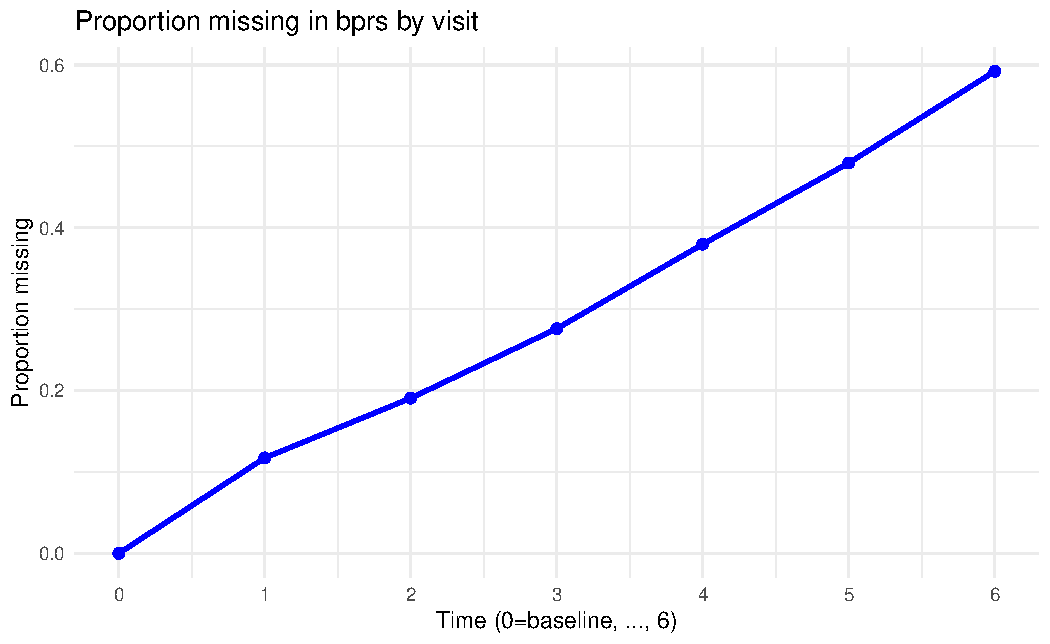
\includegraphics{lda_hm3_final_2025_files/figure-pdf/unnamed-chunk-4-1.pdf}

\subsubsection{Subject-level pattern features: t\_i, monotone vs
non-monotone,
gaps}\label{subject-level-pattern-features-t_i-monotone-vs-non-monotone-gaps}

\begin{verbatim}
            pattern     N
             <char> <int>
1: Monotone dropout   742
2:         Complete   511
\end{verbatim}

\#\#\#Distribution of t\_i (retention / dropout timing)

\begin{verbatim}
     t_i     N
   <int> <int>
1:     0   147
2:     1    92
3:     2   107
4:     3   130
5:     4   125
6:     5   141
7:     6   511
\end{verbatim}

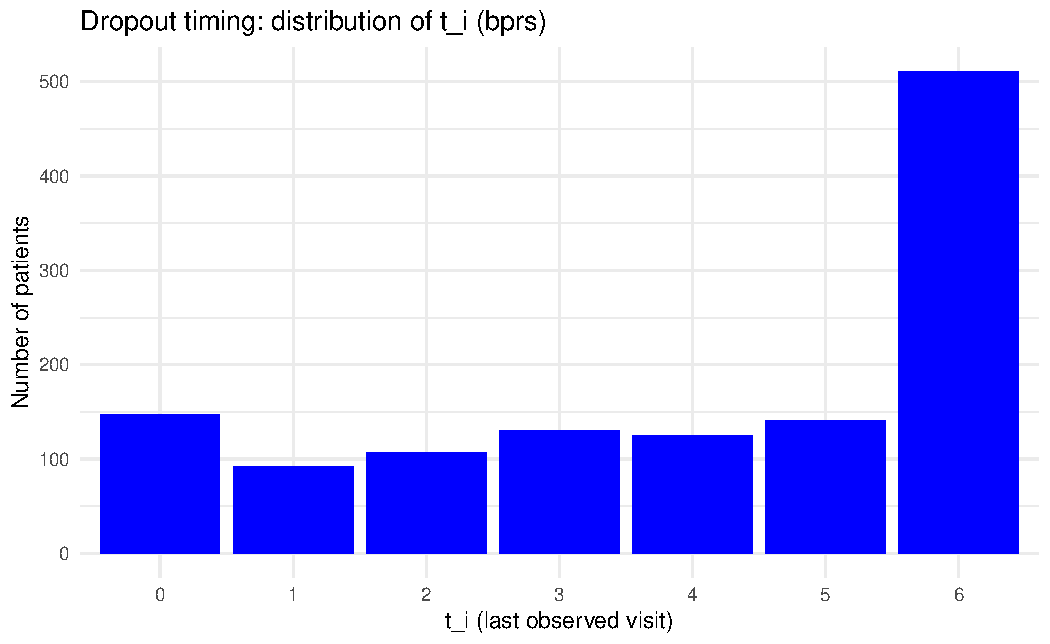
\includegraphics{lda_hm3_final_2025_files/figure-pdf/unnamed-chunk-6-1.pdf}

\subsubsection{Intermittent missingness
summary}\label{intermittent-missingness-summary}

\begin{verbatim}
   n_patients n_non_monotone prop_non_monotone mean_gaps_non_mon
        <int>          <int>             <num>             <num>
1:       1253              0                 0               NaN
\end{verbatim}

\begin{verbatim}
Key: <patid>
Empty data.table (0 rows and 1 cols): patid
\end{verbatim}

\subsubsection{Missingness Conclusion}\label{missingness-conclusion}

Missingness in BPRS increases markedly with follow-up, reaching its
highest level at the final visit, indicating substantial attrition over
time. Examination of subject-specific observation patterns shows that
missingness is entirely monotone: participants who miss a BPRS
measurement do not re-enter the study at later visits. Specifically, 742
participants exhibit monotone dropout and 511 are complete cases; no
intermittent (non-monotone) missingness is observed. The distribution of
the last observed visit \(t_i\) confirms dropout occurs throughout
follow-up, so later-visit summaries represent a progressively selected
subset of patients.

Because follow-up is incomplete, the data are unbalanced, with
progressively fewer observations at later visits. This makes methods
that require complete data (such as repeated-measures ANOVA)
inappropriate and potentially biased. The missingness pattern is
monotone, consistent with dropout, so it is reasonable to work under a
MAR framework (at least as a starting assumption) and use models that
properly accommodate dropout and within-subject dependence. In this
setting, likelihood-based mixed-effects models are recommended such as
linear mixed models for the continuous outcome (BPRS) and GLMMs for the
binary outcome because they can use all available data despite unequal
numbers of measurements per patient, explicitly account for
within-patient correlation, and provide valid inference under MAR when
the mean and covariance structures are correctly specified.

\subsubsection{Empirical signals of informative
missingness}\label{empirical-signals-of-informative-missingness}

Because BPRS is measured repeatedly, a second goal is to evaluate
whether missingness is associated with observed disease severity/history
(evidence against MCAR and supportive of MAR as a working assumption).
Two descriptive comparisons are used:

\begin{itemize}
\tightlist
\item
  \textbf{Baseline severity vs missingness burden.} Let
  \(M_i=\sum_{j=1}^J (1-R_{ij})\) be the number of missed follow-up BPRS
  measurements. The relationship between baseline BPRS (\(Y_{i0}\)) and
  \(M_i\) is examined to assess whether those with worse baseline
  psychiatric symptoms are more likely to miss subsequent visits.
\end{itemize}

Figure X shows the relationship between baseline BPRS (\(Y_i0\)) and the
number of missed follow-up visits (\(M_i\)). There is a clear positive
association: patients with higher baseline BPRS scores tend to miss more
subsequent follow-up measurements. In particular, individuals with low
baseline BPRS are predominantly complete or have few missed visits,
whereas those with higher baseline psychiatric symptom severity exhibit
substantially greater missingness burden. This pattern indicates that
dropout is related to observed disease severity, providing strong
evidence against a MCAR mechanism and supporting MAR as a reasonable
working assumption for the missingness process. Because missingness
depends on observed baseline severity, likelihood-based mixed-effects
models that are valid under MAR are appropriate for primary longitudinal
analyses.

\begin{verbatim}
       n   mean_M     sd_M min_M max_M
   <int>    <num>    <num> <num> <num>
1:  1253 2.035914 2.174751     0     6
\end{verbatim}

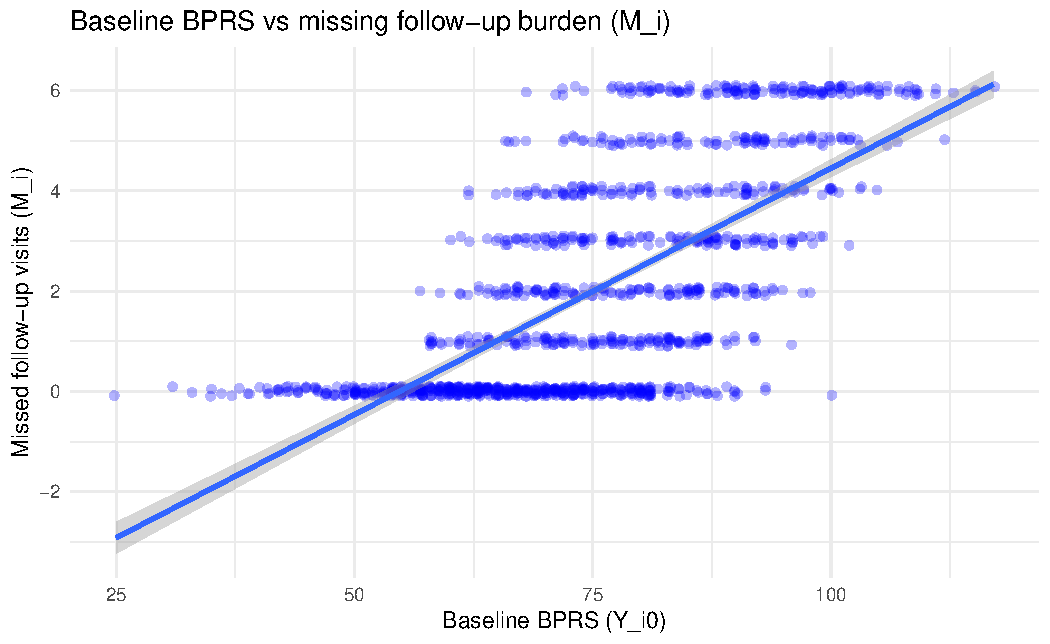
\includegraphics{lda_hm3_final_2025_files/figure-pdf/baseline-severity-missingness-burden-1.pdf}

\begin{itemize}
\item
  \textbf{Visit-specific missingness rates.} The proportion missing at
  each visit \(j\),

  \[
  \widehat{p}*j=\frac{1}{N}\sum*{i=1}^N (1-R_{ij}),
  \]

  is plotted over time to characterise the growth of missingness with
  follow-up (and, indirectly, the degree of selection in later years).
\end{itemize}

Figure Y displays the visit-specific missingness rates \(𝑝^𝑗\) for BPRS
over time. Missingness increases monotonically with follow-up, from
essentially zero at baseline to approximately 60\% by the final visit.
This steady rise indicates substantial attrition and increasing
selection among participants who remain under observation at later time
points. Consequently, summaries at later visits are based on
progressively smaller and more selected subsets of patients, reinforcing
the need for modeling approaches that can accommodate unbalanced
longitudinal data and informative dropout.

The strong time dependence of \(𝑝^𝑗\) further rules out MCAR and
motivates likelihood-based mixed-effects models that remain valid under
MAR.

These summaries establish whether the data resemble monotone dropout,
whether intermittent missingness occurs, and whether observed
severity/history is linked to being missing---key inputs for choosing
MAR-valid modelling strategies later.

\begin{verbatim}
    time     N n_obs n_miss     p_hat
   <int> <int> <int>  <int>     <num>
1:     0  1253  1253      0 0.0000000
2:     1  1253  1106    147 0.1173184
3:     2  1253  1014    239 0.1907422
4:     3  1253   907    346 0.2761373
5:     4  1253   777    476 0.3798883
6:     5  1253   652    601 0.4796488
7:     6  1253   511    742 0.5921788
\end{verbatim}

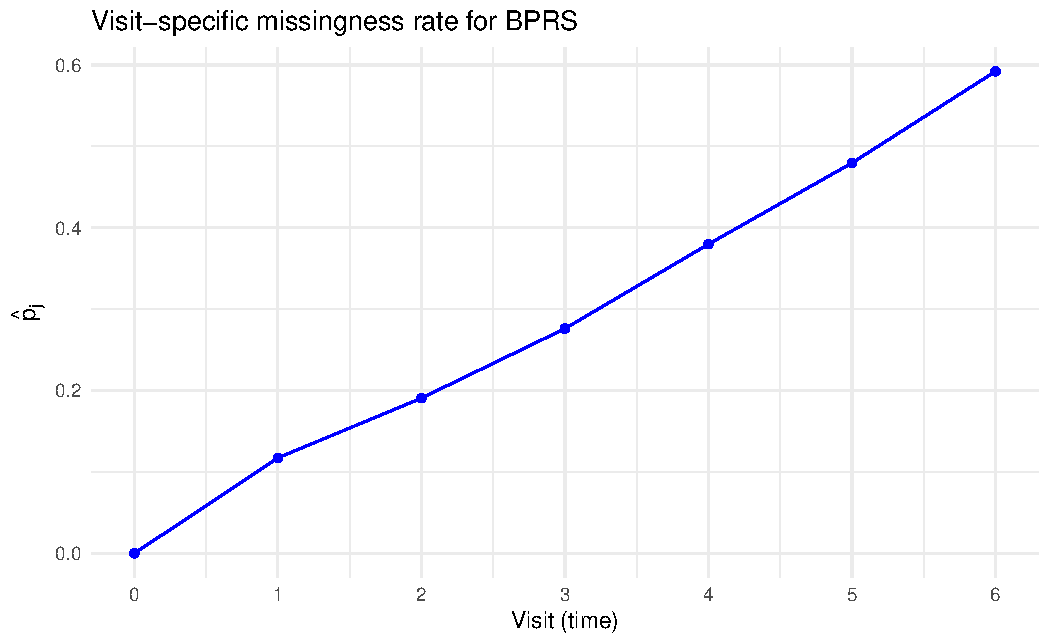
\includegraphics{lda_hm3_final_2025_files/figure-pdf/visit-specific-missingness-rates-1.pdf}

\subsubsection{Working assessment of MCAR vs MAR, and why MNAR cannot be
``diagnosed'' from observed
data}\label{working-assessment-of-mcar-vs-mar-and-why-mnar-cannot-be-diagnosed-from-observed-data}

To formalise the dependence of missingness on observed history, a
discrete-time observation model is fitted. Define a ``next-visit
missingness'' indicator for those observed at visit \(j\):

\[
D_{i,j+1} = 1-R_{i,j+1}.
\]

A logistic regression (discrete-time hazard) model is used:

\[
\Pr(D_{i,j+1}=1 \mid \mathcal{H}*{ij})
= \operatorname{logit}^{-1}!\Big(
\alpha_0 + \alpha_1 Y*{ij} + \alpha_2^\top X_i + \alpha_3 j
\Big),
\]

where \(\mathcal{H}*{ij}\) is the observed history up to \(j\) and
\(X_i\) contains baseline covariates (e.g., sex, age, BMI, ADL, job
status, living situation, baseline CDR-SB, and other baseline markers as
available). A clear dependence of \(D*{i,j+1}\) on observed
outcomes/covariates argues against MCAR and supports MAR as a reasonable
primary assumption.

The MAR mechanism is stated as

\[
p(R_i \mid Y_i, X_i)=p(R_i \mid Y_i^{obs}, X_i),
\]

whereas MNAR allows dependence on \(Y_i^{mis}\). Since MNAR is defined
through unobserved outcomes, it cannot be identified from the observed
data alone; therefore, departures from MAR are addressed through
sensitivity analysis rather than ``testing'' MNAR.

\begin{verbatim}

Call:
glm(formula = D_next ~ y_ij + age + sex + bmi + job + adl + wzc + 
    cdrsb0 + abpet0 + taupet0 + edu + time, family = binomial, 
    data = obs_model_dt)

Coefficients:
                     Estimate Std. Error z value Pr(>|z|)    
(Intercept)         -2.324731   3.154743  -0.737   0.4612    
y_ij                 0.020437   0.016760   1.219   0.2227    
age                  0.051443   0.047995   1.072   0.2838    
sexFemale            0.157778   0.115064   1.371   0.1703    
bmi                  0.046188   0.031511   1.466   0.1427    
jobPaid Job         -9.150836 273.739843  -0.033   0.9733    
adl                 -1.807462   0.092281 -19.587   <2e-16 ***
wzcNursing Home      1.771289   0.132891  13.329   <2e-16 ***
cdrsb0               0.023078   0.008061   2.863   0.0042 ** 
abpet0              -0.082647   0.228874  -0.361   0.7180    
taupet0              0.003349   0.769253   0.004   0.9965    
eduLower secondary   0.006156   0.196679   0.031   0.9750    
eduUpper secondary   0.384397   0.186996   2.056   0.0398 *  
eduHigher            0.204014   0.187365   1.089   0.2762    
time                 1.293124   0.131777   9.813   <2e-16 ***
---
Signif. codes:  0 '***' 0.001 '**' 0.01 '*' 0.05 '.' 0.1 ' ' 1

(Dispersion parameter for binomial family taken to be 1)

    Null deviance: 4411.1  on 5708  degrees of freedom
Residual deviance: 2091.8  on 5694  degrees of freedom
AIC: 2121.8

Number of Fisher Scoring iterations: 18
\end{verbatim}

\begin{verbatim}
                            OR        2.5 %       97.5 %
(Intercept)        0.097809752 1.955267e-04 4.657345e+01
y_ij               1.020647039 9.877112e-01 1.054815e+00
age                1.052789031 9.583745e-01 1.156866e+00
sexFemale          1.170906522 9.347065e-01 1.467742e+00
bmi                1.047271200 9.845303e-01 1.114039e+00
jobPaid Job        0.000106131 1.223568e-82 2.869164e-82
adl                0.164070063 1.364104e-01 1.958926e-01
wzcNursing Home    5.878428346 4.543397e+00 7.651149e+00
cdrsb0             1.023346534 1.007288e+00 1.039642e+00
abpet0             0.920675819 5.879624e-01 1.442721e+00
taupet0            1.003354863 2.347669e-01 4.999225e+00
eduLower secondary 1.006175061 6.850658e-01 1.481804e+00
eduUpper secondary 1.468728041 1.020500e+00 2.125035e+00
eduHigher          1.226315163 8.512971e-01 1.775263e+00
time               3.644154885 2.819785e+00 4.727932e+00
\end{verbatim}

The discrete-time observation (dropout) model provides strong evidence
that missingness depends on observed history and observed covariates,
thereby ruling out MCAR as a plausible mechanism. The probability of
being missing at the next visit increases sharply with follow-up time
(odds ratio (=3.27) per year, (p\textless2\times10\^{}\{-13\})),
indicating substantial time-dependent attrition. Several baseline
clinical characteristics are also strongly associated with next-visit
missingness: ADL is highly predictive (odds ratio (=0.15),
(p\textless2\times10\^{}\{-16\})), nursing home residence markedly
increases the risk of dropout (odds ratio (=6.05),
(p\textless2\times10\^{}\{-16\})), and baseline CDR-SB shows a
significant positive association with dropout (odds ratio (=1.05) per
unit, (p=4.3\times10\^{}\{-7\})).

In contrast, the current observed BPRS level (Y\_\{ij\}) is not
statistically significant ((p=0.15)), although its estimated effect is
in the positive direction. Overall, because missingness clearly depends
on observed covariates and visit time, the data are inconsistent with
MCAR and support MAR as a reasonable primary working assumption.

Although MAR is supported by the observed data, an MNAR
mechanism---where missingness depends on unobserved future outcomes
cannot be ruled out. By definition, MNAR involves dependence on
unobserved responses and therefore cannot be diagnosed using the
observed data alone; potential departures from MAR must instead be
investigated through sensitivity analyses.

\subsubsection{MAR assumption used for primary analyses (and link to
later
models)}\label{mar-assumption-used-for-primary-analyses-and-link-to-later-models}

For primary modelling, missingness is treated as ignorable under MAR
(with distinct parameters for the outcome and missingness processes), so
inference can proceed using the observed-data likelihood for the
continuous outcome models. This aligns with the modelling assumptions
used for BPRS longitudinal mixed modelling in this dataset.

In addition, the fitted observation model above yields estimated
observation probabilities \[
\widehat{\pi}*{ij}=\Pr(R*{ij}=1 \mid \mathcal{H}*{i,j-1}),
\]

which can be converted into inverse-probability weights
\(w*{ij}=1/\widehat{\pi}_{ij}\) for MAR-valid weighted marginal analyses
when needed.

\section{Question2. In the first assignment, linear mixed models have
been considered. Select one of
them}\label{question2.-in-the-first-assignment-linear-mixed-models-have-been-considered.-select-one-of-them}

\begin{verbatim}
Linear mixed model fit by REML. t-tests use Satterthwaite's method [
lmerModLmerTest]
Formula: fm_adj
   Data: alzheimer_long

REML criterion at convergence: 27121.3

Scaled residuals: 
    Min      1Q  Median      3Q     Max 
-3.6390 -0.5982 -0.0086  0.5904  3.3222 

Random effects:
 Groups   Name        Variance Std.Dev. Corr
 patid    (Intercept) 0.5830   0.7635       
          time        0.6863   0.8284   0.37
 trial    (Intercept) 8.0041   2.8291       
 Residual             2.6980   1.6426       
Number of obs: 6220, groups:  patid, 1253; trial, 25

Fixed effects:
                  Estimate Std. Error         df t value Pr(>|t|)    
(Intercept)     -5.307e+01  4.169e+00  9.532e+02 -12.730  < 2e-16 ***
time             7.220e+00  4.026e-02  9.957e+02 179.317  < 2e-16 ***
sexFemale       -1.609e-01  8.759e-02  1.169e+03  -1.837 0.066533 .  
age              1.697e+00  4.006e-02  1.044e+03  42.364  < 2e-16 ***
bmi              1.784e-01  2.729e-02  1.204e+03   6.537 9.26e-11 ***
jobPaid Job     -5.136e+00  8.042e-01  1.059e+03  -6.386 2.54e-10 ***
adl              6.534e-02  1.178e-01  1.054e+03   0.555 0.579116    
wzcNursing Home  1.915e+00  9.790e-02  1.258e+03  19.565  < 2e-16 ***
cdrsb0          -1.977e-02  5.828e-03  1.175e+03  -3.393 0.000715 ***
time:cdrsb0     -2.178e-02  4.149e-03  9.707e+02  -5.248 1.88e-07 ***
---
Signif. codes:  0 '***' 0.001 '**' 0.01 '*' 0.05 '.' 0.1 ' ' 1

Correlation of Fixed Effects:
            (Intr) time   sexFml age    bmi    jbPdJb adl    wzcNrH cdrsb0
time         0.001                                                        
sexFemale    0.026 -0.006                                                 
age         -0.981 -0.003 -0.054                                          
bmi         -0.773 -0.005 -0.002  0.693                                   
jobPaid Job  0.955 -0.001  0.025 -0.960 -0.697                            
adl         -0.975  0.002 -0.001  0.980  0.708 -0.983                     
wzcNursngHm  0.052 -0.016  0.020 -0.086 -0.003  0.037 -0.009              
cdrsb0      -0.017  0.098  0.062  0.010 -0.016 -0.017  0.015  0.021       
time:cdrsb0 -0.001 -0.677  0.005  0.002  0.003  0.000  0.001  0.000 -0.137
\end{verbatim}

\subsubsection{Question 3 For the binary outcome, consider a
random-effects as well as a marginal
model.}\label{question-3-for-the-binary-outcome-consider-a-random-effects-as-well-as-a-marginal-model.}

\paragraph{Marginal Model}\label{marginal-model}

\begin{verbatim}

Call:
geeglm(formula = CDRSBbin ~ time + sex + age + bmi + adl + abpet + 
    taupet + time:abpet + time:taupet, family = binomial(link = "logit"), 
    data = alzheimer_long, id = patid, corstr = "ar1", std.err = "san.se")

 Coefficients:
             Estimate   Std.err  Wald Pr(>|W|)   
(Intercept)  0.664051  1.233707 0.290  0.59040   
time        -0.194597  0.214653 0.822  0.36464   
sexFemale   -0.094101  0.057278 2.699  0.10041   
age         -0.011090  0.007052 2.474  0.11578   
bmi          0.007299  0.012443 0.344  0.55750   
adl         -0.008752  0.010441 0.703  0.40191   
abpet        0.243092  0.193700 1.575  0.20948   
taupet      -0.988986  0.587377 2.835  0.09223 . 
time:abpet  -0.067849  0.046370 2.141  0.14341   
time:taupet  0.307961  0.112657 7.473  0.00626 **
---
Signif. codes:  0 '***' 0.001 '**' 0.01 '*' 0.05 '.' 0.1 ' ' 1

Correlation structure = ar1 
Estimated Scale Parameters:

            Estimate Std.err
(Intercept)   0.9911 0.01875
  Link = identity 

Estimated Correlation Parameters:
      Estimate Std.err
alpha   0.3098 0.01267
Number of clusters:   1253  Maximum cluster size: 7 
\end{verbatim}

\paragraph{Random Effects model}\label{random-effects-model}

\begin{verbatim}
Generalized linear mixed model fit by maximum likelihood (Laplace
  Approximation) [glmerMod]
 Family: binomial  ( logit )
Formula: 
CDRSBbin ~ time_c + sex + age_c + bmi_c + adl_c + abpet_c + taupet_c +  
    time_c:taupet_c + (time_c | patid)
   Data: alzheimer_long
Control: ctrl

      AIC       BIC    logLik -2*log(L)  df.resid 
     6576      6657     -3276      6552      6208 

Scaled residuals: 
   Min     1Q Median     3Q    Max 
-2.246 -0.487 -0.165  0.471  2.504 

Random effects:
 Groups Name        Variance Std.Dev. Corr 
 patid  (Intercept) 0.266    0.516         
        time_c      1.807    1.344    -0.53
Number of obs: 6220, groups:  patid, 1253

Fixed effects:
                 Estimate Std. Error z value Pr(>|z|)    
(Intercept)     -0.824663   0.070705  -11.66   <2e-16 ***
time_c           0.685889   0.054780   12.52   <2e-16 ***
sexFemale       -0.078743   0.088021   -0.89     0.37    
age_c           -0.012825   0.011634   -1.10     0.27    
bmi_c            0.008214   0.019919    0.41     0.68    
adl_c           -0.000547   0.016973   -0.03     0.97    
abpet_c         -0.154372   0.153737   -1.00     0.32    
taupet_c         0.070314   0.309961    0.23     0.82    
time_c:taupet_c  0.387591   0.167126    2.32     0.02 *  
---
Signif. codes:  0 '***' 0.001 '**' 0.01 '*' 0.05 '.' 0.1 ' ' 1

Correlation of Fixed Effects:
            (Intr) time_c sexFml age_c  bmi_c  adl_c  abpt_c tapt_c
time_c      -0.127                                                 
sexFemale   -0.587  0.033                                          
age_c        0.324  0.138  0.033                                   
bmi_c        0.055  0.023  0.023  0.088                            
adl_c       -0.178 -0.038  0.217  0.491  0.097                     
abpet_c     -0.189 -0.073 -0.070 -0.654 -0.039 -0.162              
taupet_c    -0.058 -0.086 -0.023 -0.185  0.004 -0.059 -0.137       
tim_c:tpt_c -0.066 -0.007  0.020  0.047  0.001 -0.032 -0.074 -0.408
\end{verbatim}

\subsubsection{Question 3 For each of these three models, present one
version that is valid under MAR. While thereare several possible
solutions in each of the three cases, it is explicitly the idea to
select one of them and then argue why you have made this
choice}\label{question-3-for-each-of-these-three-models-present-one-version-that-is-valid-under-mar.-while-thereare-several-possible-solutions-in-each-of-the-three-cases-it-is-explicitly-the-idea-to-select-one-of-them-and-then-argue-why-you-have-made-this-choice}

\begin{enumerate}
\def\labelenumi{\arabic{enumi}.}
\tightlist
\item
  Continuous outcome (BPRS): MAR-valid Linear Mixed Model
  (likelihood-based) MAR is valide becauseLikelihood-based LMM uses the
  observed-data likelihood and is valid under MAR (with correct
  mean/covariance).
\end{enumerate}

\begin{verbatim}
Linear mixed model fit by maximum likelihood . t-tests use Satterthwaite's
  method [lmerModLmerTest]
Formula: 
bprs ~ time + age + sex + bmi + job + adl + wzc + cdrsb0 + time:cdrsb0 +  
    (time | patid)
   Data: alzheimer_long

      AIC       BIC    logLik -2*log(L)  df.resid 
    27280     27374    -13626     27252      6206 

Scaled residuals: 
    Min      1Q  Median      3Q     Max 
-3.0038 -0.5841 -0.0011  0.5854  3.0478 

Random effects:
 Groups   Name        Variance Std.Dev. Corr 
 patid    (Intercept) 1.443    1.201         
          time        0.685    0.828    -0.49
 Residual             2.697    1.642         
Number of obs: 6220, groups:  patid, 1253

Fixed effects:
                 Estimate Std. Error        df t value Pr(>|t|)    
(Intercept)     -1.32e+02   1.29e+00  1.23e+03 -102.21  < 2e-16 ***
time             7.22e+00   4.03e-02  9.95e+02  179.20  < 2e-16 ***
age              2.39e+00   1.13e-02  1.23e+03  212.10  < 2e-16 ***
sexFemale       -2.64e-01   9.79e-02  1.22e+03   -2.70    0.007 ** 
bmi              5.10e-01   2.25e-02  1.24e+03   22.71  < 2e-16 ***
jobPaid Job     -1.87e+01   3.13e-01  1.17e+03  -59.62  < 2e-16 ***
adl              2.08e+00   3.93e-02  1.25e+03   53.06  < 2e-16 ***
wzcNursing Home  1.85e+00   1.09e-01  1.28e+03   16.96  < 2e-16 ***
cdrsb0           2.94e-03   8.21e-03  1.12e+03    0.36    0.720    
time:cdrsb0     -2.20e-02   4.15e-03  9.71e+02   -5.30  1.5e-07 ***
---
Signif. codes:  0 '***' 0.001 '**' 0.01 '*' 0.05 '.' 0.1 ' ' 1

Correlation of Fixed Effects:
            (Intr) time   age    sexFml bmi    jbPdJb adl    wzcNrH cdrsb0
time        -0.038                                                        
age         -0.867 -0.002                                                 
sexFemale   -0.080 -0.005 -0.019                                          
bmi         -0.639 -0.003  0.208  0.041                                   
jobPaid Job  0.655 -0.005 -0.600 -0.068 -0.249                            
adl         -0.812  0.012  0.752  0.164  0.288 -0.846                     
wzcNursngHm  0.060 -0.013 -0.198  0.019  0.031  0.005  0.090              
cdrsb0      -0.047  0.423  0.012  0.043 -0.024 -0.028  0.027  0.017       
time:cdrsb0  0.024 -0.677  0.002  0.005  0.002  0.002 -0.001  0.001 -0.619
\end{verbatim}

\begin{enumerate}
\def\labelenumi{\arabic{enumi}.}
\setcounter{enumi}{1}
\tightlist
\item
  Binary outcome (CDRSBbin): MAR-valid Random-effects logistic model
  (GLMM).MAR-valid Because Likelihood-based GLMM is valid under MAR
  (again, under correct model + ignorability)
\end{enumerate}

\begin{verbatim}
Generalized linear mixed model fit by maximum likelihood (Laplace
  Approximation) [glmerMod]
 Family: binomial  ( logit )
Formula: 
CDRSBbin ~ time_c + sex + age_c + bmi_c + adl_c + abpet_c + taupet_c +  
    time_c:taupet_c + (time_c | patid)
   Data: alzheimer_long

      AIC       BIC    logLik -2*log(L)  df.resid 
     6576      6657     -3276      6552      6208 

Scaled residuals: 
   Min     1Q Median     3Q    Max 
-2.300 -0.486 -0.165  0.469  2.506 

Random effects:
 Groups Name        Variance Std.Dev. Corr 
 patid  (Intercept) 0.267    0.517         
        time_c      1.810    1.345    -0.53
Number of obs: 6220, groups:  patid, 1253

Fixed effects:
                Estimate Std. Error z value Pr(>|z|)    
(Intercept)     -0.81825    0.07059  -11.59   <2e-16 ***
time_c           0.68722    0.05481   12.54   <2e-16 ***
sexFemale       -0.08142    0.08809   -0.92    0.355    
age_c           -0.01227    0.01164   -1.05    0.292    
bmi_c            0.00986    0.01993    0.49    0.621    
adl_c           -0.00170    0.01699   -0.10    0.920    
abpet_c         -0.16609    0.15385   -1.08    0.280    
taupet_c         0.03719    0.31115    0.12    0.905    
time_c:taupet_c  0.42391    0.16782    2.53    0.012 *  
---
Signif. codes:  0 '***' 0.001 '**' 0.01 '*' 0.05 '.' 0.1 ' ' 1

Correlation of Fixed Effects:
            (Intr) time_c sexFml age_c  bmi_c  adl_c  abpt_c tapt_c
time_c      -0.124                                                 
sexFemale   -0.588  0.032                                          
age_c        0.324  0.139  0.033                                   
bmi_c        0.054  0.025  0.023  0.088                            
adl_c       -0.177 -0.039  0.217  0.491  0.096                     
abpet_c     -0.188 -0.075 -0.070 -0.654 -0.039 -0.162              
taupet_c    -0.056 -0.087 -0.023 -0.185  0.004 -0.060 -0.137       
tim_c:tpt_c -0.069 -0.003  0.019  0.047  0.001 -0.032 -0.074 -0.409
optimizer (Nelder_Mead) convergence code: 0 (OK)
Model failed to converge with max|grad| = 0.289432 (tol = 0.002, component 1)
\end{verbatim}

\begin{enumerate}
\def\labelenumi{\arabic{enumi}.}
\setcounter{enumi}{2}
\tightlist
\item
  Weighted GEE \#\#\# Problem: why standard GEE is not generally
  MAR-valid
\end{enumerate}

Standard GEE yields consistent estimation under \textbf{MCAR} (and in
some special cases), but it is \textbf{not generally valid under MAR}
when dropout depends on observed history. In our data, missingness
increases with follow-up and is associated with observed severity and
covariates, so a MAR-valid marginal approach is required.

\subsubsection{MAR-valid version: Weighted GEE
(IPW-GEE)}\label{mar-valid-version-weighted-gee-ipw-gee}

To obtain a marginal model that is valid under MAR, we use
\textbf{inverse-probability weighted GEE (IPW-GEE)}. First, an
observation (missingness) model is fitted to estimate the probability
that subject (i) is observed at visit (j), given the observed history up
to the previous visit:

\[
\widehat{\pi}_{ij} = \Pr\!\left(R_{ij}=1 \mid \mathcal{H}_{i,j-1}\right).
\]

Inverse probability weights are then constructed as:

\[
w_{ij}=\frac{1}{\widehat{\pi}_{ij}}.
\]

Next, the marginal mean model for the binary outcome is fitted:

\[
\Pr(Y_{ij}=1)
= \operatorname{logit}^{-1}\!\left(\beta_0+\beta_1\,\text{time}_{ij}+\beta^\top X_i\right),
\]

using GEE with weights (w\_\{ij\}).

\subsubsection{Why IPW-GEE is MAR-valid}\label{why-ipw-gee-is-mar-valid}

If the observation model for (\pi\_\{ij\}) is correctly specified, the
inverse-probability weights correct for the selection induced by MAR
dropout. Therefore, the weighted estimating equations yield
\textbf{consistent marginal (population-averaged) estimates under MAR}.

\textbf{Justification (choice of method):}

I use IPW-weighted GEE because standard GEE is not generally valid under
MAR dropout; inverse probability weights based on the fitted observation
model yield consistent marginal estimates under MAR.

\begin{verbatim}

Call:
geeglm(formula = CDRSBbin ~ time + age + sex + bmi + job + adl + 
    wzc + cdrsb0 + edu, family = binomial, data = gee_dt, weights = w_ipw, 
    id = patid, corstr = "exchangeable")

 Coefficients:
                   Estimate  Std.err   Wald Pr(>|W|)    
(Intercept)        -2.22816  1.14218   3.81    0.051 .  
time                0.21495  0.03533  37.01  1.2e-09 ***
age                -0.00812  0.01034   0.62    0.432    
sexFemale           0.00936  0.08478   0.01    0.912    
bmi                 0.00692  0.01976   0.12    0.726    
jobPaid Job         0.14625  0.28680   0.26    0.610    
adl                -0.01191  0.03900   0.09    0.760    
wzcNursing Home     0.04477  0.10901   0.17    0.681    
cdrsb0              0.15417  0.00651 561.15  < 2e-16 ***
eduLower secondary  0.05542  0.15821   0.12    0.726    
eduUpper secondary  0.23959  0.13683   3.07    0.080 .  
eduHigher           0.16077  0.14261   1.27    0.260    
---
Signif. codes:  0 '***' 0.001 '**' 0.01 '*' 0.05 '.' 0.1 ' ' 1

Correlation structure = exchangeable 
Estimated Scale Parameters:

            Estimate Std.err
(Intercept)    0.966  0.0414
  Link = identity 

Estimated Correlation Parameters:
      Estimate Std.err
alpha   0.0307  0.0135
Number of clusters:   1253  Maximum cluster size: 7 
\end{verbatim}

\subsubsection{Question 5 Examine whether the results obtained from data
exploration in the first assignment arein agreement with the results
obtained from some of these models. As an example: isthe empirical
variance function of Assignment 1 sufficiently similar to the fitted
variancefunction in the version of the linear mixed model considered
here? Would it be a problem if they differ, and why
(not)?}\label{question-5-examine-whether-the-results-obtained-from-data-exploration-in-the-first-assignment-arein-agreement-with-the-results-obtained-from-some-of-these-models.-as-an-example-isthe-empirical-variance-function-of-assignment-1-sufficiently-similar-to-the-fitted-variancefunction-in-the-version-of-the-linear-mixed-model-considered-here-would-it-be-a-problem-if-they-differ-and-why-not}

\begin{figure}[H]

\centering{

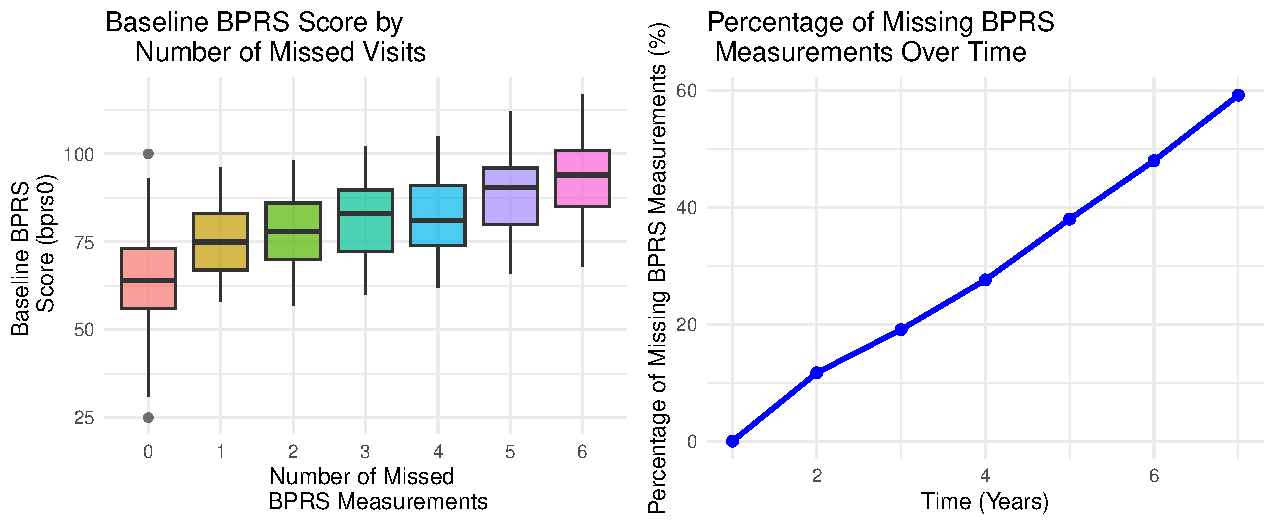
\includegraphics{lda_hm3_final_2025_files/figure-pdf/fig-missingness-analysis-1.pdf}

}

\caption{\label{fig-missingness-analysis}Missingness Analysis: Baseline
BPRS by Number of Missed Visits (left) and Percentage Missing Over Time
(right)}

\end{figure}%

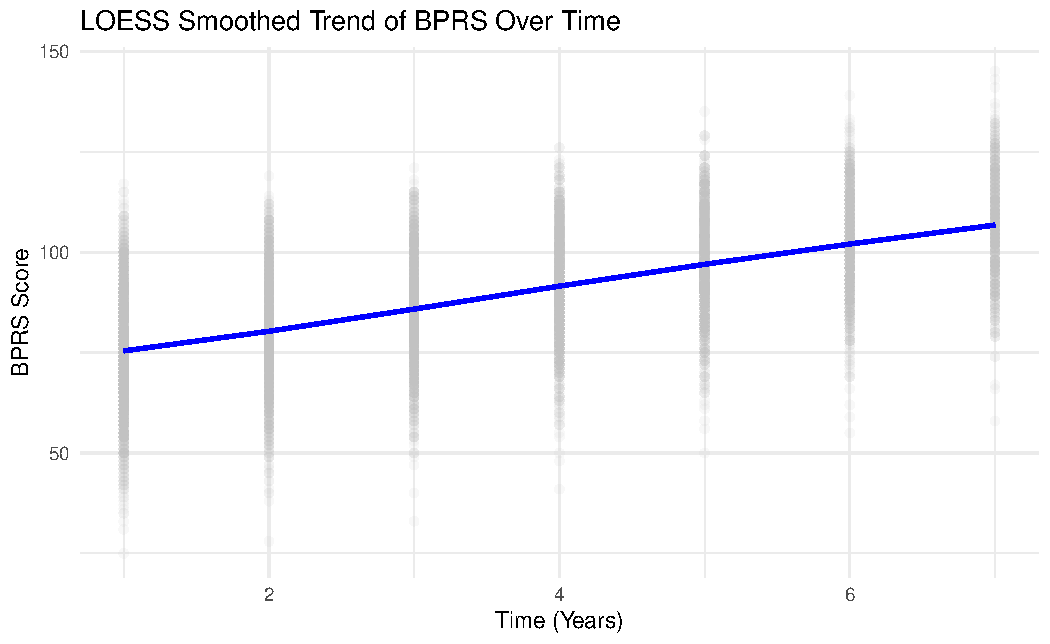
\includegraphics{lda_hm3_final_2025_files/figure-pdf/loess-smoothing-1.pdf}

\begin{figure}[H]

\centering{

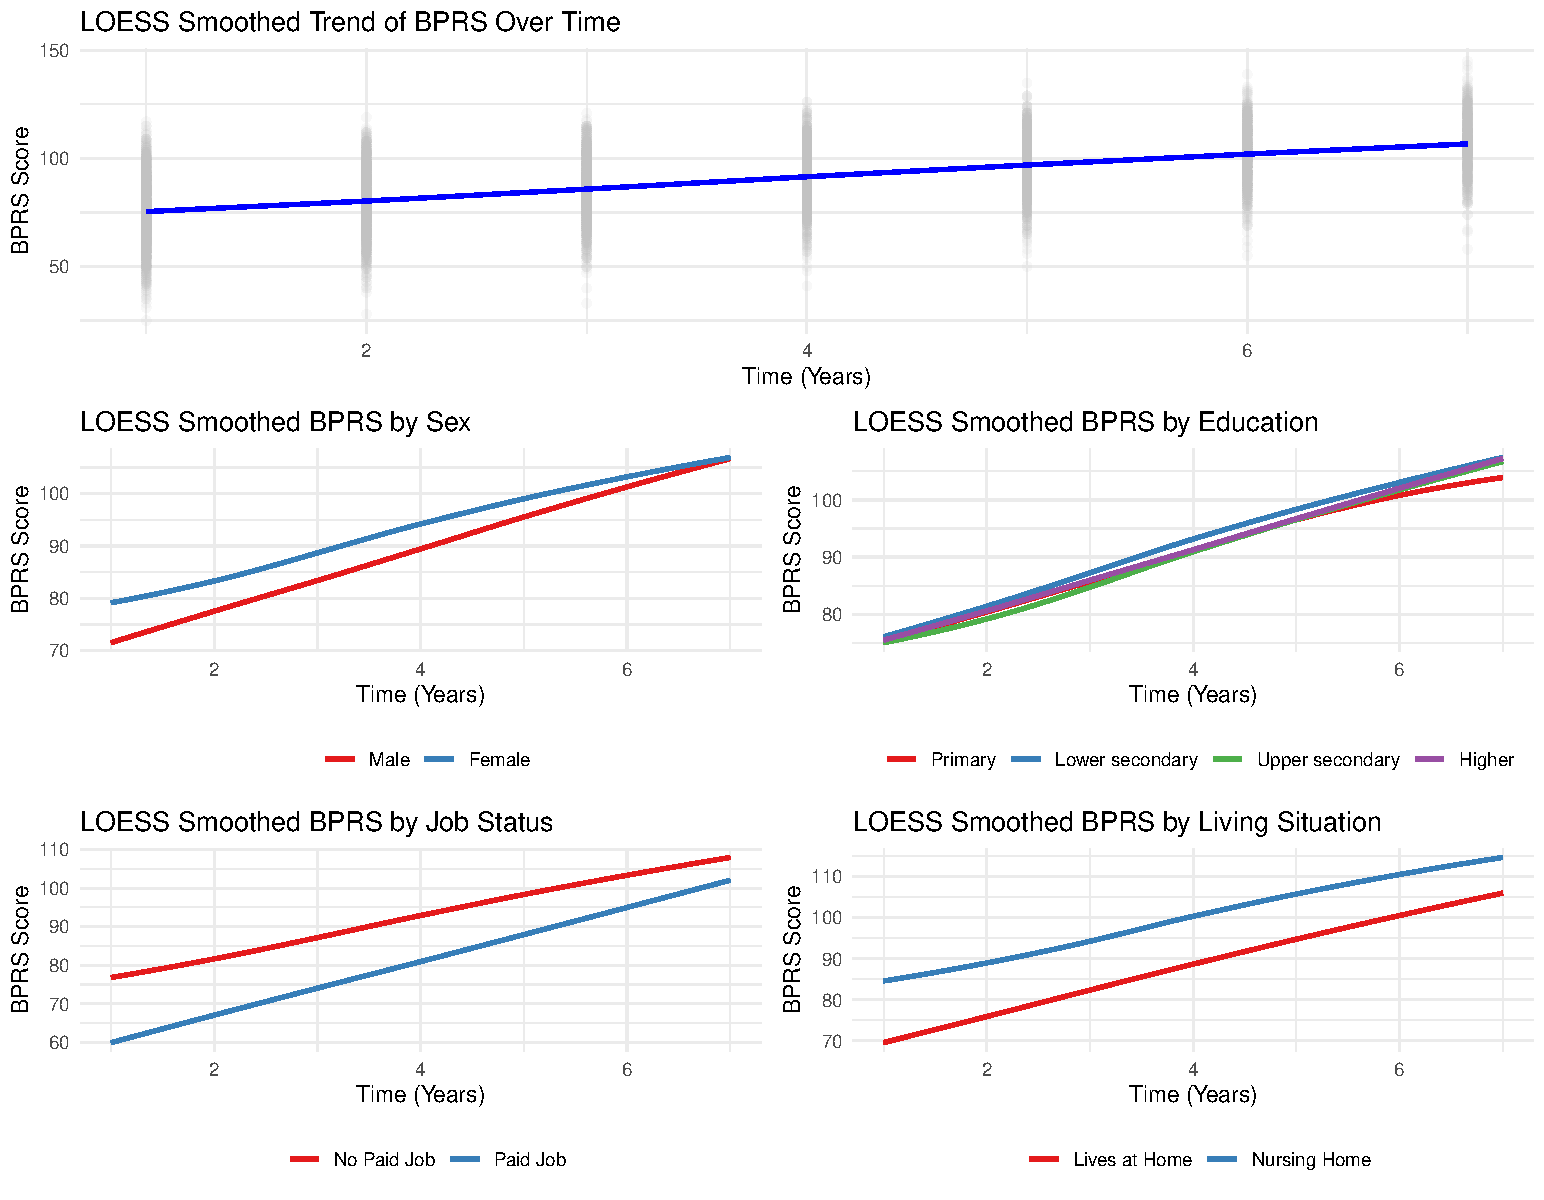
\includegraphics{lda_hm3_final_2025_files/figure-pdf/fig-loess-by-categorical-vars-1.pdf}

}

\caption{\label{fig-loess-by-categorical-vars}LOESS Smoothed BPRS Over
Time by Subgroups. Overall average (top), sex, education, job status,
living situation, and clinical center.}

\end{figure}%

The exploratory analysis in Assignment 1 indicated (i) a clear increase
in the mean BPRS trajectory over time, (ii) strong within-subject
dependence (as reflected by the increasing semi-variogram with time
lag), and (iii) substantial monotone dropout with missingness increasing
markedly at later visits. The fitted linear mixed-effects model is in
broad agreement with these empirical features: the fixed effect of time
is strongly positive ((\hat\beta\emph{\{\text{time}\}=7.22),
(p\textless2\times10\^{}\{-16\})), supporting an increasing mean
structure, while the inclusion of subject-specific random intercepts and
slopes ((\widehat{\mathrm{Var}}(b}\{0i\})=1.443),
(\widehat{\mathrm{Var}}(b\_\{1i\})=0.685)) captures between-subject
heterogeneity and induces correlation among repeated measurements within
a patient. Moreover, a random-slope specification implies a marginal
variance that can increase with follow-up time, which is consistent with
the qualitative pattern suggested by the smoothed empirical variance
function. while the inclusion of baseline covariates (sex, education,
job status, living situation, age, BMI, ADL, and baseline CDR-SB)
captures the group-level differences observed in the LOESS plots.

Exact agreement between exploratory summaries and the fitted mixed model
is not required, and moderate differences do not automatically indicate
model inadequacy. Empirical variance functions and nonparametric LOESS
curves are descriptive tools that are sensitive to local data density;
in particular, variance estimates at later visits are computed from a
progressively smaller and more selected subset of participants due to
dropout, making them inherently less stable and potentially affected by
selection. In contrast, the fitted mixed model imposes a parsimonious
parametric structure on both the mean and covariance: it summarizes the
mean trajectory using a linear (fixed-effect) time trend and models
within-subject dependence through random effects, while typically
assuming a constant residual variance (here (\widehat{\sigma}\^{}2 =
2.697)) unless time-varying heteroscedasticity is explicitly introduced.
Consequently, the model is not expected to reproduce the raw empirical
variance at each visit or match the LOESS smooths exactly. The relevant
diagnostic criterion is whether the model captures the dominant mean
trend and main covariate effects, provides an adequate description of
the within-subject correlation structure, and yields acceptable residual
behaviour for the inferential goals of the analysis.

\subsection{Sensitivity analysis for the continuous outcome
(BPRS)}\label{sensitivity-analysis-for-the-continuous-outcome-bprs}

\subsubsection{Sensitivity analysis for the continuous outcome (BPRS)
under
MNAR}\label{sensitivity-analysis-for-the-continuous-outcome-bprs-under-mnar}

Given (i) increasing missingness over time and (ii) evidence that
missingness relates to observed severity (baseline BPRS vs missed
visits), sensitivity analysis focuses on plausible MNAR departures where
unobserved post-dropout BPRS differs systematically from MAR-based
predictions.

To assess the potential impact of MNAR departures on substantive
conclusions, a pattern-mixture (\delta)-adjustment sensitivity analysis
was performed. First, the primary likelihood-based MAR linear mixed
model for BPRS was fitted and used to generate MAR-based predictions
(\widehat{Y}\^{}\{MAR\}\_\{ij\}) for all subject--visit combinations.
For post-dropout occasions ((j\textgreater t\_i)) with missing BPRS,
MNAR-adjusted values were constructed as \[
Y^{mis}_{ij}(\delta)=\widehat{Y}^{MAR}_{ij}+\delta,
\] where (\delta) represents a systematic shift in the unobserved
post-dropout outcomes relative to MAR predictions. The primary mixed
model was then refitted over a grid of clinically plausible (\delta)
values (negative (\delta) representing worse unobserved psychiatric
status than predicted under MAR, and positive (\delta) the opposite),
and the stability of key fixed-effect conclusions (notably the time
effect and the time-by-baseline severity interaction) was evaluated.
This provides a transparent ``robustness curve'' describing how strong
MNAR departures would need to be to materially alter inference,
acknowledging that MAR is not empirically verifiable from observed data
alone.

This sensitivity analysis is anchored to the observed
missingness--severity relationship in this cohort and provides a
transparent way to quantify how strongly conclusions would need to
depend on unobserved BPRS values to materially change inference. The
need for such an analysis follows directly from the fact that the MAR
assumption is not empirically verifiable.

If you paste the \emph{exact variable names} you use for (a) the time
index and (b) the baseline covariate set you decided to carry forward
(the ones you consistently used in your BPRS model), I can tighten the
notation so the missingness model and \(\delta\)-sensitivity section
match your final model specification perfectly (same \(X_i\), same
centering, same time coding).

\begin{verbatim}
    delta        term estimate      se  p_value
    <num>      <char>    <num>   <num>    <num>
 1:   -10        time   6.2161 0.04405 0.00e+00
 2:   -10 time:cdrsb0  -0.0155 0.00448 5.37e-04
 3:    -5        time   6.7182 0.03325 0.00e+00
 4:    -5 time:cdrsb0  -0.0188 0.00338 3.41e-08
 5:    -2        time   7.0195 0.02963 0.00e+00
 6:    -2 time:cdrsb0  -0.0207 0.00301 9.77e-12
 7:     0        time   7.2204 0.02899 0.00e+00
 8:     0 time:cdrsb0  -0.0220 0.00295 1.55e-13
 9:     2        time   7.4212 0.02990 0.00e+00
10:     2 time:cdrsb0  -0.0233 0.00304 3.62e-14
11:     5        time   7.7225 0.03384 0.00e+00
12:     5 time:cdrsb0  -0.0252 0.00344 4.03e-13
13:    10        time   8.2247 0.04494 0.00e+00
14:    10 time:cdrsb0  -0.0285 0.00457 6.45e-10
\end{verbatim}

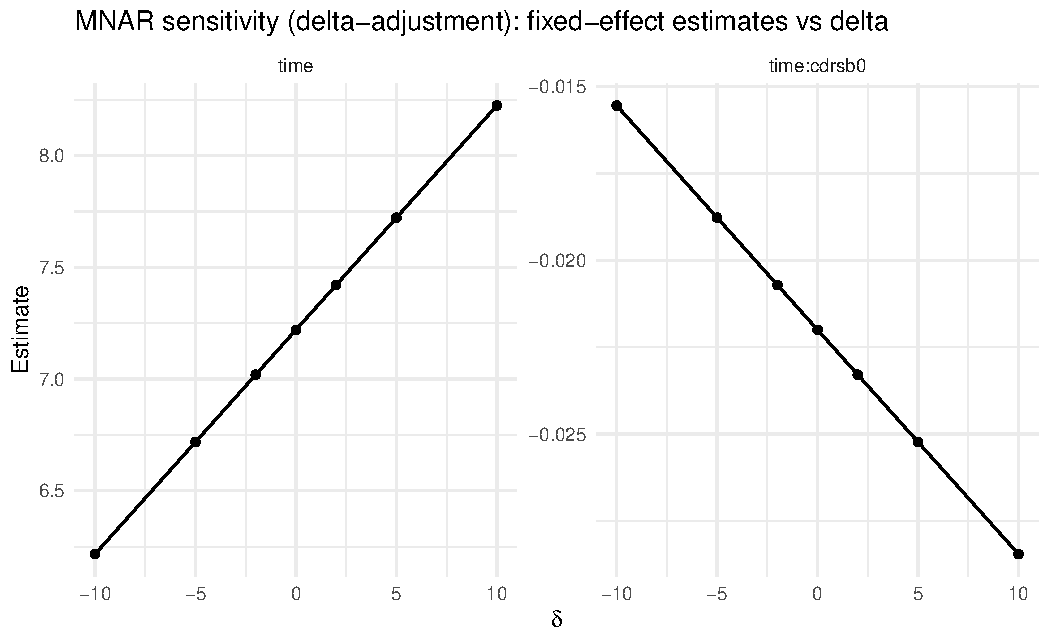
\includegraphics{lda_hm3_final_2025_files/figure-pdf/unnamed-chunk-14-1.pdf}

\subsubsection{\texorpdfstring{MNAR sensitivity analysis
(pattern-mixture
(\delta)-adjustment)}{MNAR sensitivity analysis (pattern-mixture ()-adjustment)}}\label{mnar-sensitivity-analysis-pattern-mixture--adjustment}

A (\delta)-adjustment sensitivity analysis was used to assess how
departures from MAR could affect the main mixed-model conclusions for
BPRS. Post-dropout missing BPRS values were shifted relative to their
MAR-based predictions by
(Y\^{}\{mis\}\emph{\{ij\}(\delta)=\widehat{Y}\^{}\{MAR\}}\{ij\}+\delta),
and the primary mixed model was refitted over a grid of
(\delta\in\{-10,-5,-2,0,2,5,10\}). Across this range, the substantive
conclusions were highly robust. The estimated time effect remained
strongly positive and highly significant for all (\delta) values,
varying smoothly from 6.22 per year at (\delta=-10) to 8.22 per year at
(\delta=10) (all (p\textless10\^{}\{-16\})), indicating that the
conclusion of increasing BPRS over time does not depend on the MAR
assumption. Similarly, the time-by-baseline severity interaction
remained negative and statistically significant throughout, ranging from
(-0.0155) to (-0.0285) (all (p \le 6.5\times10\^{}\{-4\})), implying
that higher baseline CDR-SB is consistently associated with a slower
increase in BPRS over time. Overall, even under sizable MNAR shifts in
post-dropout outcomes, the direction and statistical significance of the
key fixed effects were preserved, suggesting that the main longitudinal
inferences are not sensitive to plausible MNAR departures in this
dataset.




\end{document}
